% !TEX program = xelatex
\documentclass{beamer}
    \usepackage{hyperref}
    \usepackage{seqsplit}
    \urlstyle{same}
    \graphicspath{{imgs/}}
    \usetheme{metropolis} 

    \title{DRM Considered Harmful}
    \date{April 20, 2018}
    \author{Bernardo Meurer}
    \institute{Santa Barbara City College}

\begin{document}
\maketitle

\begin{frame}{whoami}
	\begin{columns}[T]
		\begin{column}{.5\textwidth}
			\begin{block}{}
				\begin{itemize}
					\item Bernardo Meurer
					\item Computer Science student
					\item Intern @ Standard Cognition \url{http://standard.ai}
					\item \texttt{\small{meurerbernardo@gmail.com}}
					\item \url{http://meurer.xyz/}
				\end{itemize}
			\end{block}
		\end{column}

		\begin{column}{.5\textwidth}
			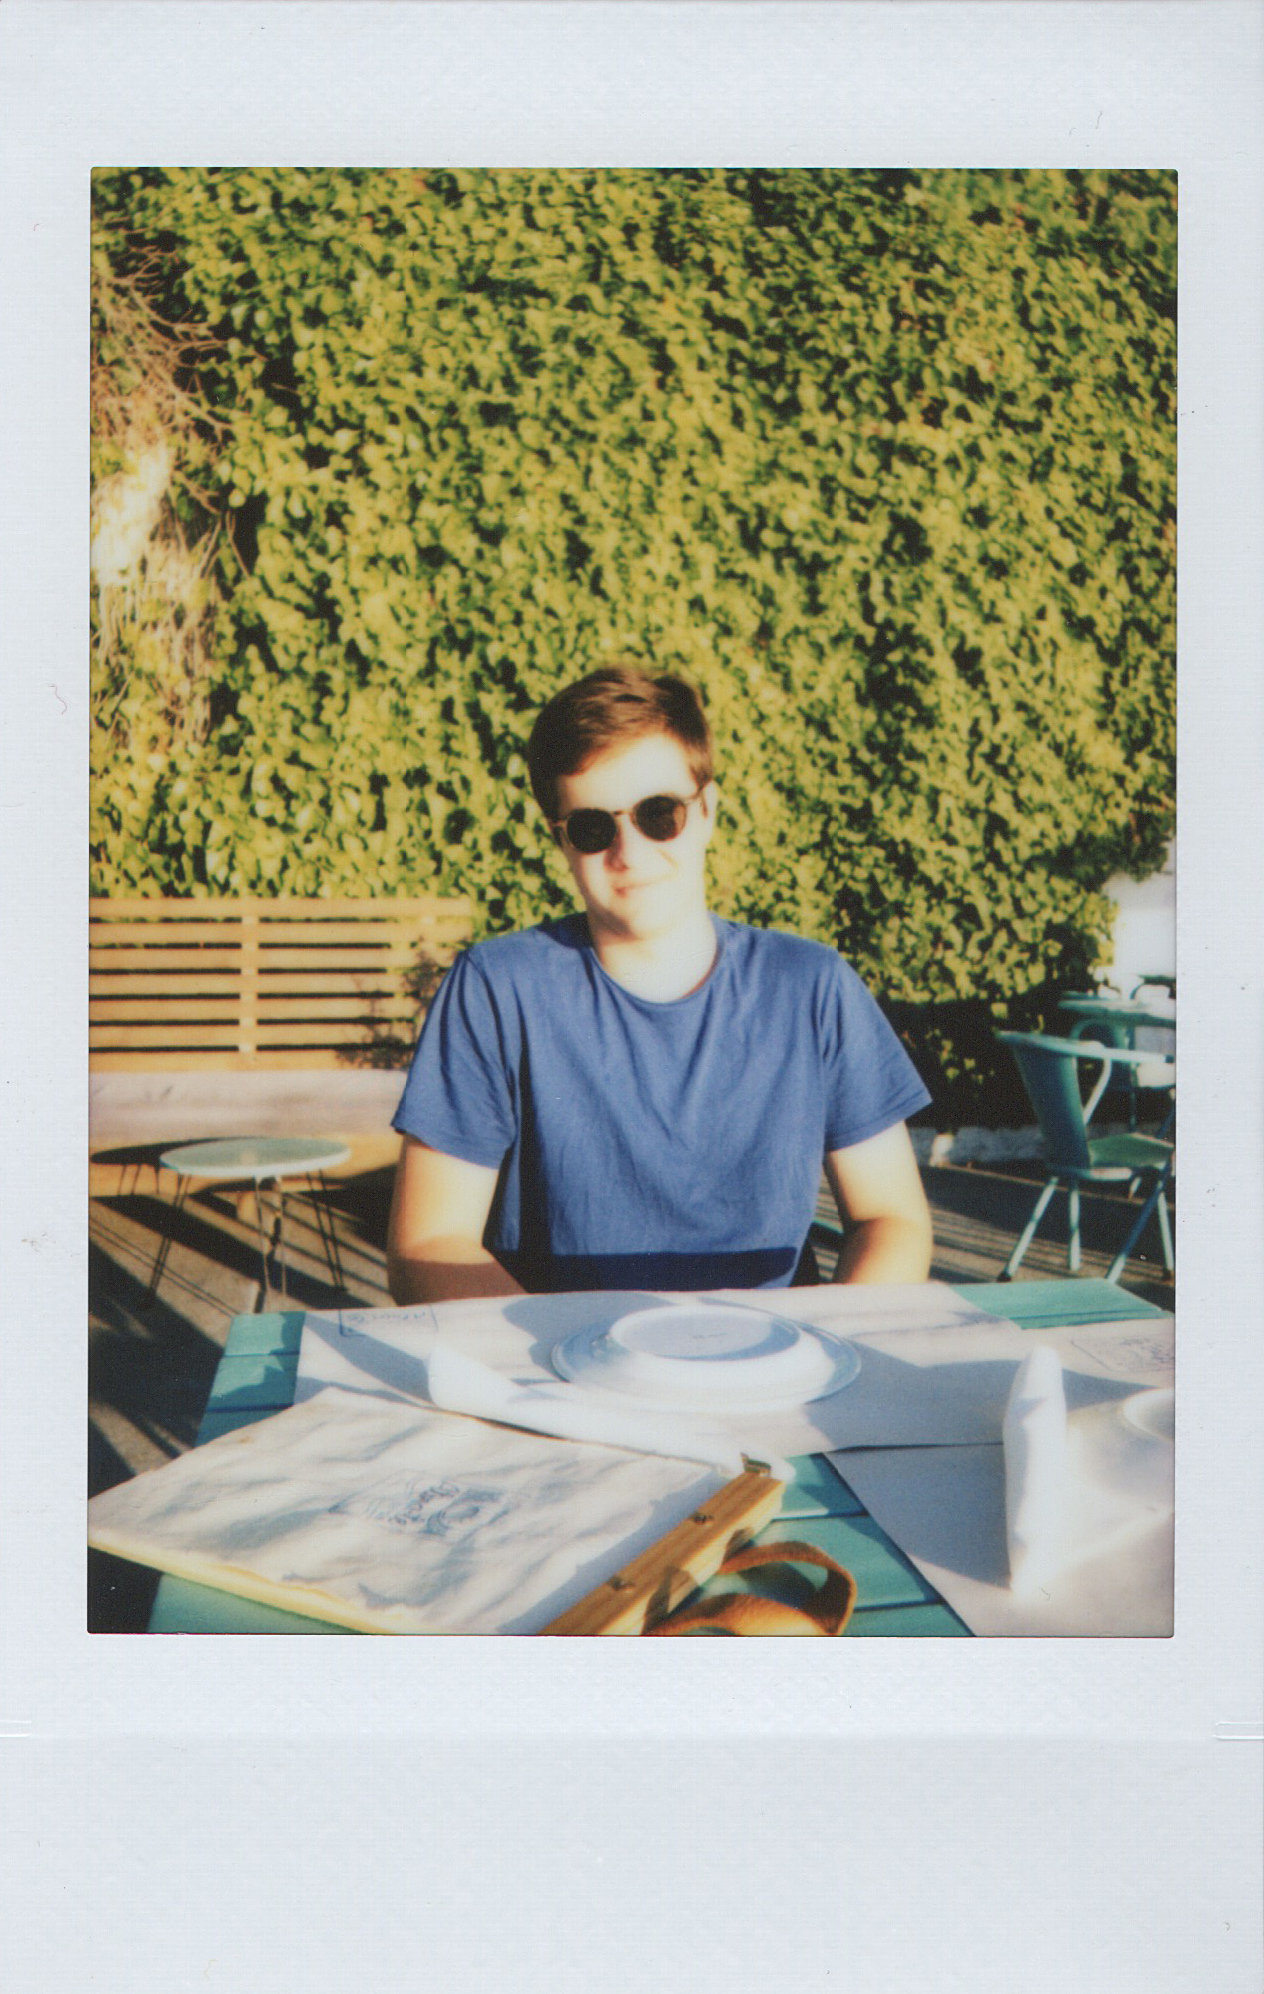
\includegraphics[width=\textwidth]{me.jpg}
		\end{column}
	\end{columns}
\end{frame}

\begin{frame}{DR-What?}
	\setbeamercovered{dynamic}
	\begin{itemize}
		\item What's DRM?\@\pause{}
		      \begin{itemize}
			      \item Digital Rights Management\pause{}
		      \end{itemize}
		\item Examples
		      \begin{itemize}
			      \item CD's \pause{}
			      \item DVD's \pause{}
			      \item Netflix, iTunes, Hulu, etc
		      \end{itemize}
	\end{itemize}
\end{frame}

\begin{frame}[t]{DVD --- The first culprit}
	\begin{itemize}
		\item Content Scramble System (CSS)\pause{}
		\item Did it work?
		      \begin{itemize}
			      \item \pause{}It failed miserably
		      \end{itemize}
    \end{itemize}
    \vfill
\end{frame}

\begin{frame}{DVD --- The first culprit}
	\begin{figure}
		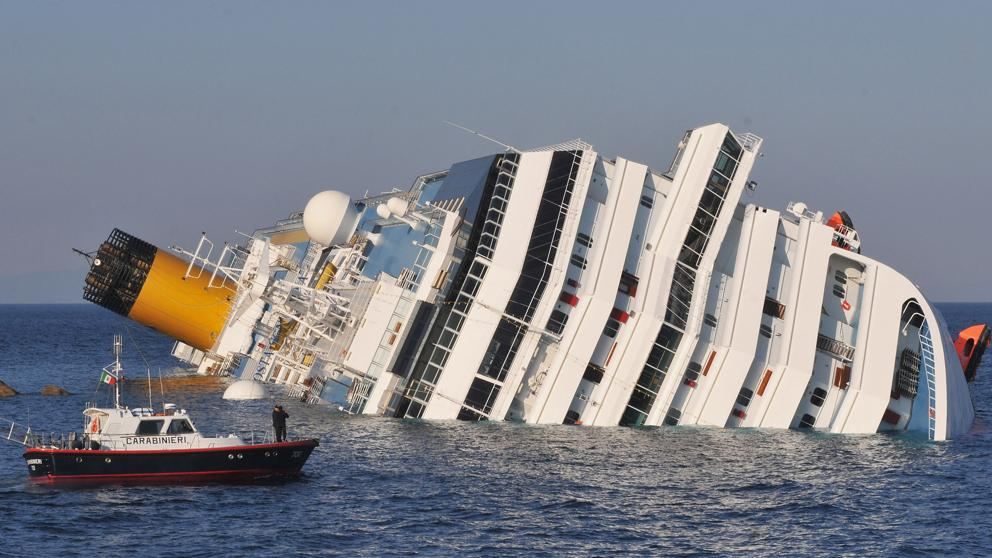
\includegraphics[width=\textwidth]{fail1.jpg}
	\end{figure}
\end{frame}

\begin{frame}{DVD --- The first culprit}
	\begin{itemize}
		\item Content Scramble System (CSS)
		\item Did it work?
		      \begin{itemize}
			      \item It failed miserably
			      \item DeCSS\pause{}
		      \end{itemize}
		\item What did the companies do?\pause{}
		      \begin{itemize}
			      \item Sue\pause{}
		      \end{itemize}
		\item What did people do?\pause{}
		      \begin{itemize}
			      \item Get creative\pause{}
			      \item Steganography\pause{}
			      \item Way too many web protocols\pause{}
			      \item T-shirts\pause{}
			      \item MIDI files\pause{}
			      \item Poems --- A 456-stanza haiku! \url{https://www.cs.cmu.edu/~dst/DeCSS/Gallery/decss-haiku.txt}\pause{}
			      \item Prime numbers?
		      \end{itemize}
	\end{itemize}
\end{frame}

\begin{frame}{This presentation is illegal}
    \scriptsize
	\(\seqsplit{4856507896573978293098418946942861377074420873513579240196520736 6869851340104723744696879743992611751097377770102744752804905883 1384037549709987909653955227011712157025974666993240226834596619 6060348517424977358468518855674570257125474999648219418465571008 4119086259716947970799152004866709975923596061320725973797993618 8606316914473588300245336972781813914797955513399949394882899846 9178361001825978901031601961835034344895687053845208538045842415 6548248893338047475871128339598968522325446084089711197712769412 0795862440547161321005006459820176961771809478113622002723448272 2493232595472346880029277764979061481298404283457201463489685471 6908235473783566197218622496943162271666393905543024156473292485 5248991225739466548627140482117138124388217717602984125524464744 5055834628144883356319027253195904392838737640739168912579240550 1562088978716337599910788708490815909754801928576845198859630532 3823490558092032999603234471140776019847163531161713078576084862 2363702835701049612595681846785965333100770179916146744725492728 3348691600064758591746278121269007351830924153010630289329566584 3662000800476778967984382090797619859493646309380586336721469695 9750279687712057249966669805614533820741203159337703099491527469 1835659376210222006812679827344576093802030447912277498091795593 8387121000588766689258448700470772552497060444652127130404321182 610103591186476662963858495087448497373476861420880529443}
	\)
\end{frame}

\begin{frame}{DVD --- The first culprit}
	\begin{figure}
		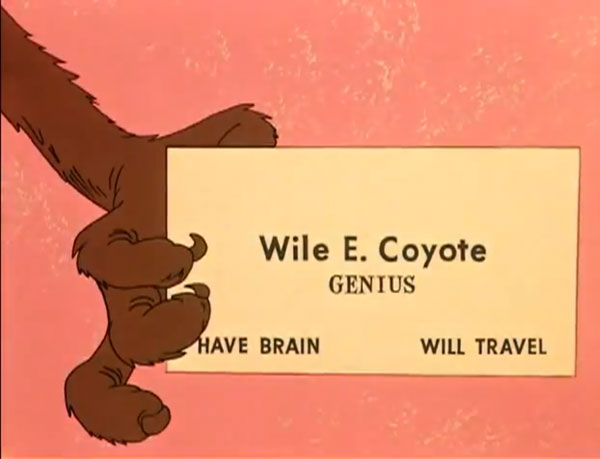
\includegraphics[width=\textwidth]{fail2.jpg}
	\end{figure}
\end{frame}

\begin{frame}{DRM --- A dream}
    \begin{itemize}
        \item DRM is a copyright owner's dream\pause{}
        \item (Un?) Fortunately users don't feel the same way\ldots\pause{}
        \item Not one DRM scheme of interest has survived
        \begin{itemize}
            \item Some smaller schemes are unbroken, such as the one protecting so-called ``Super Audio CD's'' (SACD).\pause{}
        \end{itemize}
        \item So after \(\approx \)35 years of trying \ldots nothing.\pause{}
        \item If the entertainment industry can't do it \ldots\pause{}
        \item Who can?
    \end{itemize}
\end{frame}

\begin{frame}{DRM --- A dream}
    \Huge
    \vfill
    \centering
    nobody
    \vfill
\end{frame}

\begin{frame}{DRM --- More than annoying}
    \begin{itemize}
        \item It's not about being a nuisance\pause{}
        \item It's about your rights and your freedom\pause{}
        \item DRM infringes on your right to privacy
    \end{itemize}
\end{frame}

\begin{frame}{Property --- What and how}
    \begin{itemize}
        \item ``The Labor of one's Body and the Work of his Hands, we may say, are properly his.'' --- John Locke\pause{}
        \item We appropriate something from the common by applying labor onto it.\pause{}
        \item Appropriation is only valid insofar as it leaves ``enough, and as good'' of the common to the community.\pause{}
        \item What does this mean?
        \begin{itemize}
            \item If you pick apples in the forest, those apples are yours.\pause{}
            \item You can't appropriate the sun\pause{}
            \item or the ocean, or the atmosphere.
        \end{itemize}
    \end{itemize}
\end{frame}

\begin{frame}{Property --- What and how}
    \begin{itemize}
        \item How does Intellectual Property work then?\pause{}
        \item Property is fundamentally more than the result of one's labor\pause{}
        \item It is rather the expression of Man's personality (Hegel).\pause{}
        \item Intellectual property is just another form of property, since it's an expression of its author's personality
    \end{itemize}
\end{frame}

\begin{frame}{Intellectual Property and copying}
    \begin{itemize}
        \item Copying harms the owner, even if it doesn't deprive him of his creation.\pause{}
        \item So in the same way we have laws against stealing, we should have laws against copying\pause{}
        \item We do! It's called Copyright!
    \end{itemize}
\end{frame}

\begin{frame}{Copyright}
    \begin{itemize}
        \item Copyright tries to join two opposing sides:\pause{}
        \begin{itemize}
            \item Protecting the author\pause{}
            \item Protecting the public\pause{}
        \end{itemize}
        \item But why does the public need protection?\pause{}
        \begin{itemize}
            \item So that the common cannot be improperly appropriated!\pause{}
            \item Would it be reasonable if someone started charging royalties for the happy birthday song? What about the alphabet?\pause{}
            \item What about royalties on ancient Greek philosophy? Or if someone copyrighted multiplication?\pause{}
        \end{itemize}
    \end{itemize}
\end{frame}

\begin{frame}{Copyright}
    \begin{itemize}
        \item It's clear that these things make no sense\ldots\pause{}
        \item But why?\pause{}
        \item In the same way there is a common of things, there is a common of ideas, of intangibles\pause{}
        \item Copyright's job is to protect that, above all.
    \end{itemize}
\end{frame}

\begin{frame}{Common of Ideas}
    \begin{itemize}
        \item What makes the common of ideas?\pause{}
        \item Mostly things that belong in the public domain.\pause{}
        \item But also culture itself
        \begin{itemize}
            \item Current events
            \item Things that pertain to the public\pause{}
        \end{itemize} 
        \item Imagine if someone tried to own 4th of July
        
    \end{itemize}
\end{frame}

\begin{frame}{Made with Free Software!}
	This presentation was made using Free (as in Freedom) and Open Source software!
	\begin{itemize}
		\item Vim
		\item \LaTeX{} + Beamer + \texttt{metropolis}
		\item Evince
	\end{itemize}
	Learn more about software that respects you and your rights at \url{https://www.gnu.org/}
\end{frame}
\end{document}